%!TEX root = ../Chapter3.tex
\begin{figure*}[t!]
 \centering
 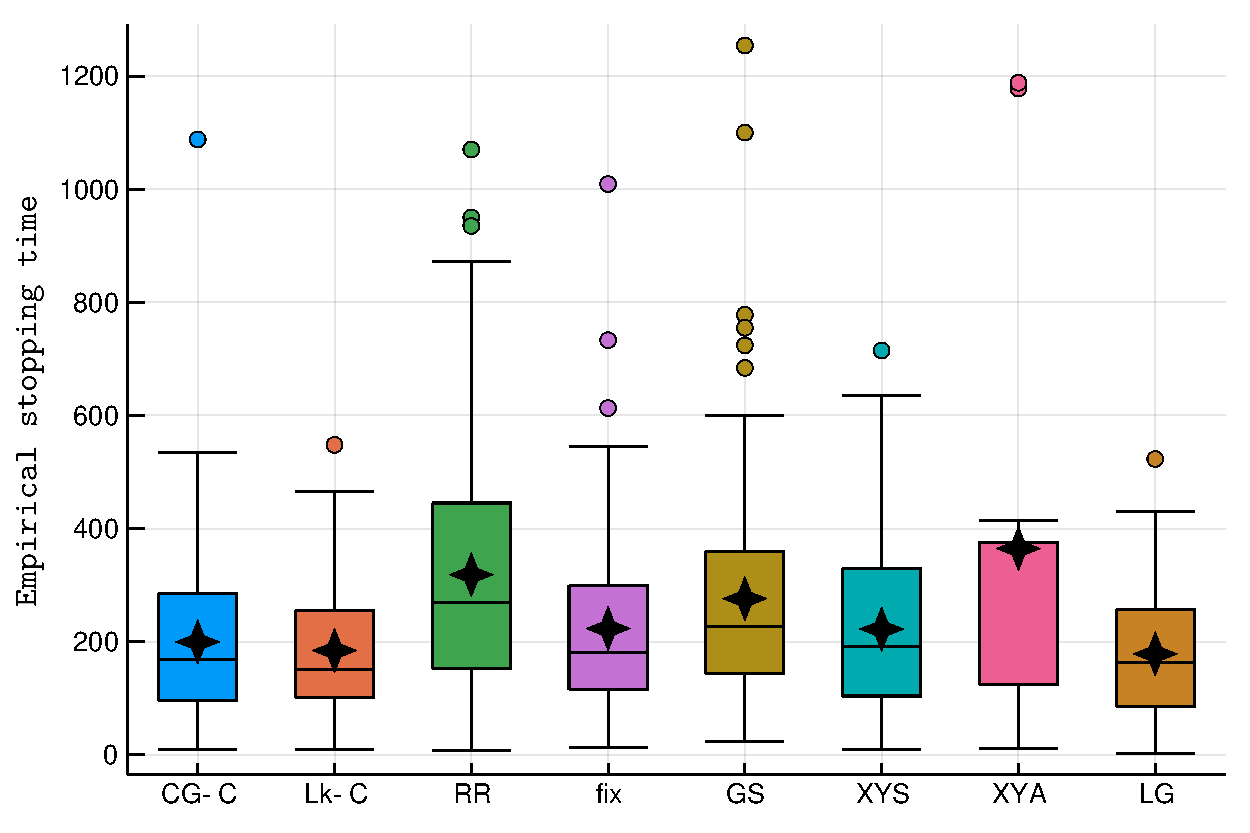
\includegraphics[clip, width= 0.3\textwidth]{Chapter3/img/bai_sin_0-1}
 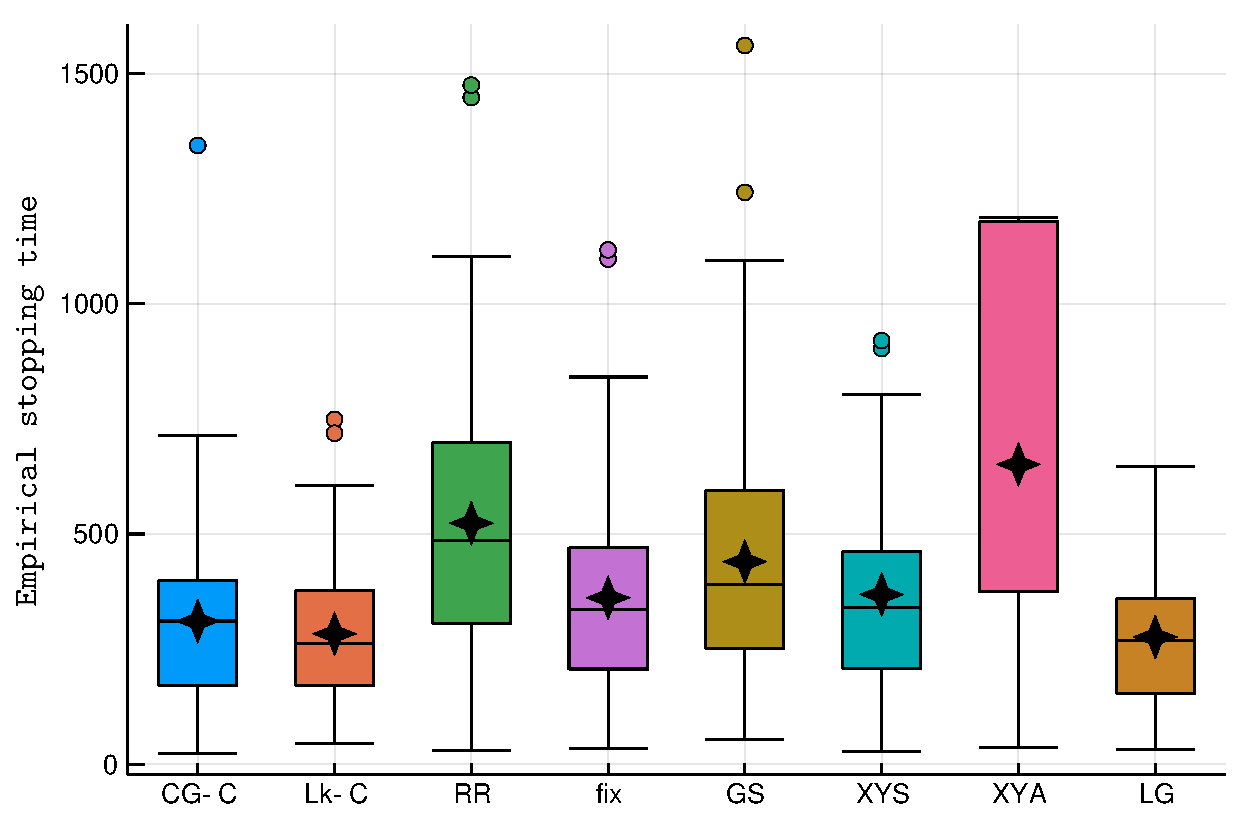
\includegraphics[clip, width= 0.3\textwidth]{Chapter3/img/bai_sin_0-01}
 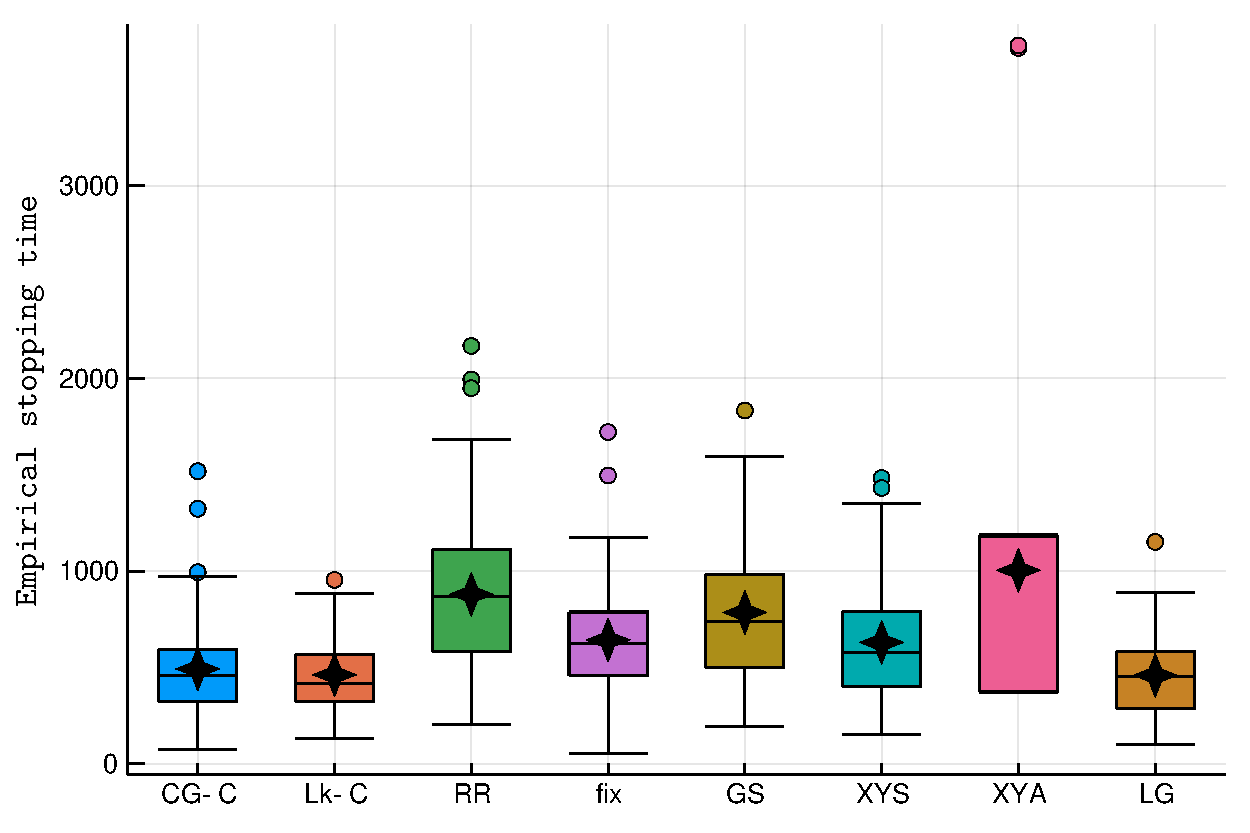
\includegraphics[clip, width= 0.3\textwidth]{Chapter3/img/bai_sin_0-0001}
 \caption{Sample complexity of different linear BAI sampling rules over the usual counter-example with $\delta=0.1, 0.01, 0.0001$ respectively. CG = \LGC,  Lk = \LG, RR = uniform sampling, fix = tracking the fixed weights, GS = \XYS with $\gopt$-allocation, XYS = \XYS with $\xyopt$-allocation, LG = \LGapE. The mean stopping time is represented by a black cross.}
 \label{fig:sample_complexity_1}
\end{figure*}

\begin{figure*}[t!]
 \centering
 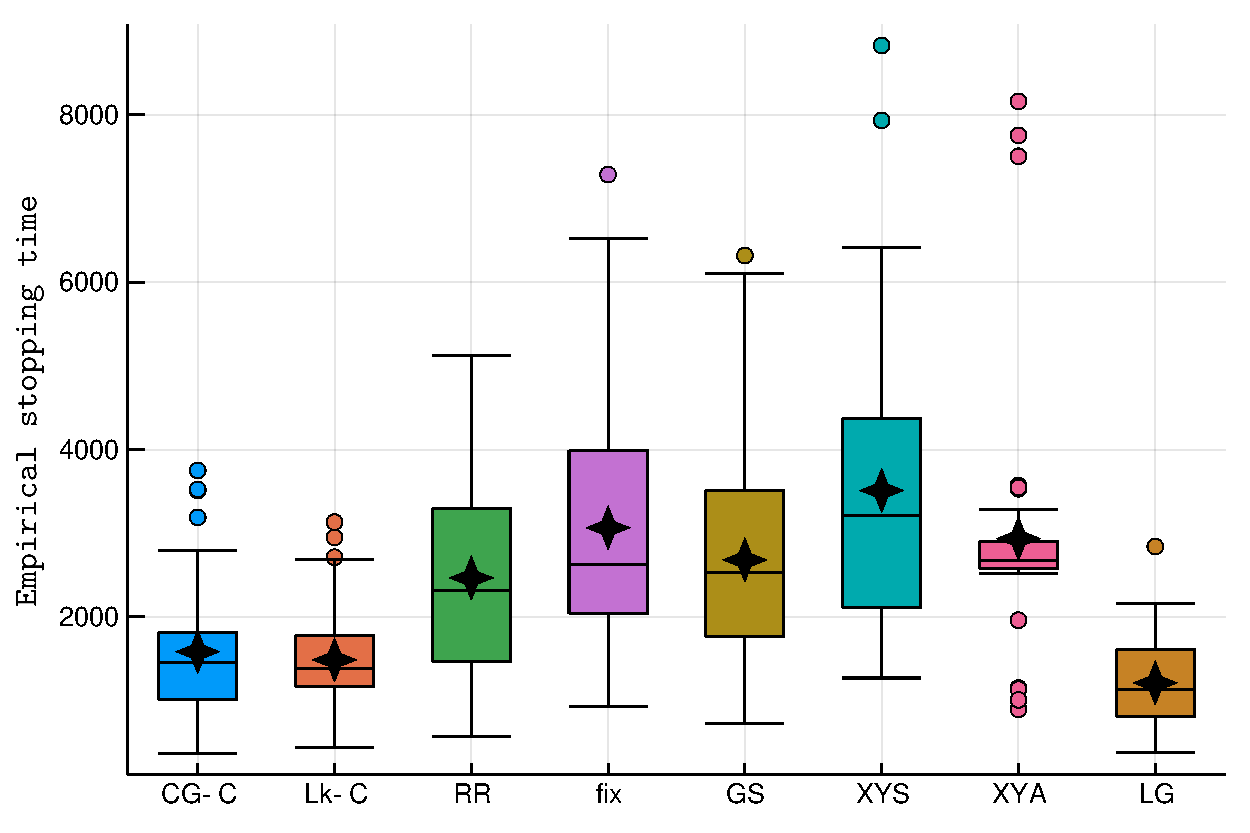
\includegraphics[clip, width= 0.24\textwidth]{Chapter3/img/bai_dim_6}
 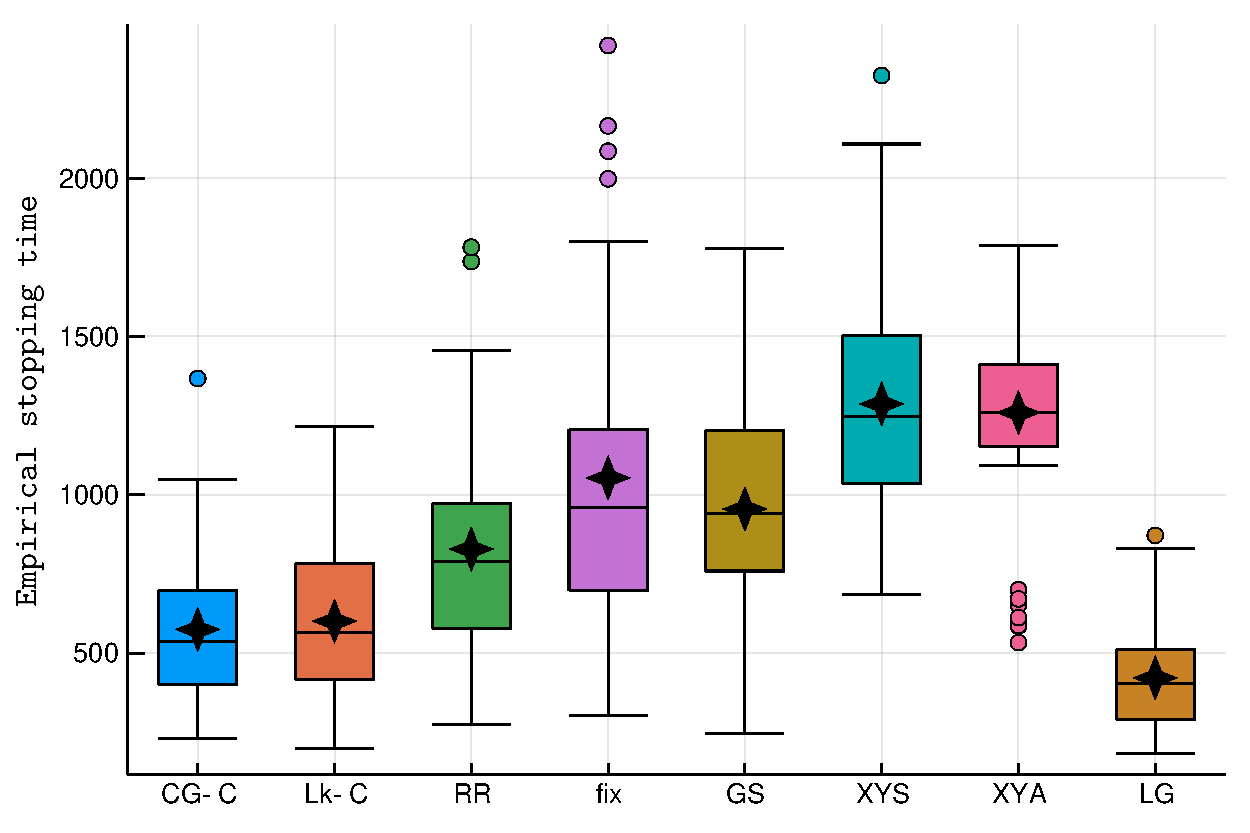
\includegraphics[clip, width= 0.24\textwidth]{Chapter3/img/bai_dim_8}
 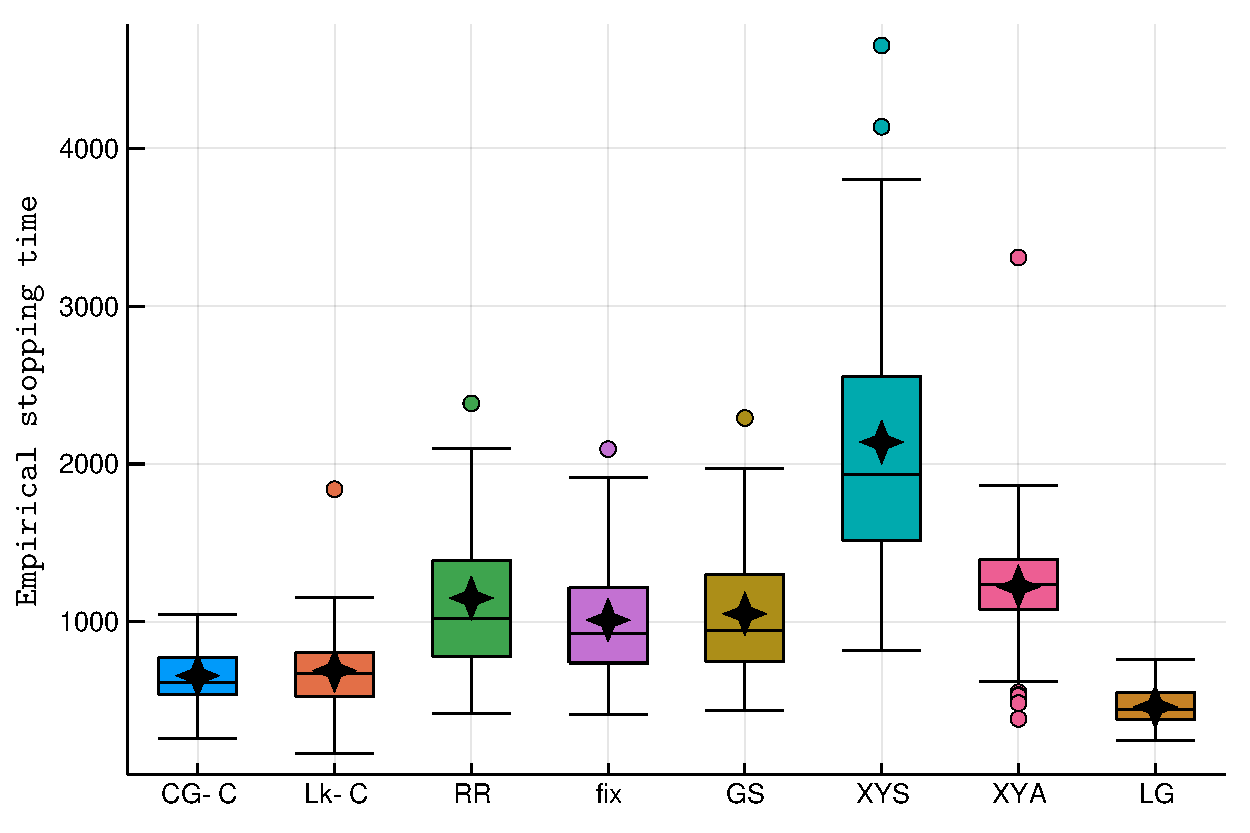
\includegraphics[clip, width= 0.24\textwidth]{Chapter3/img/bai_dim_10}
 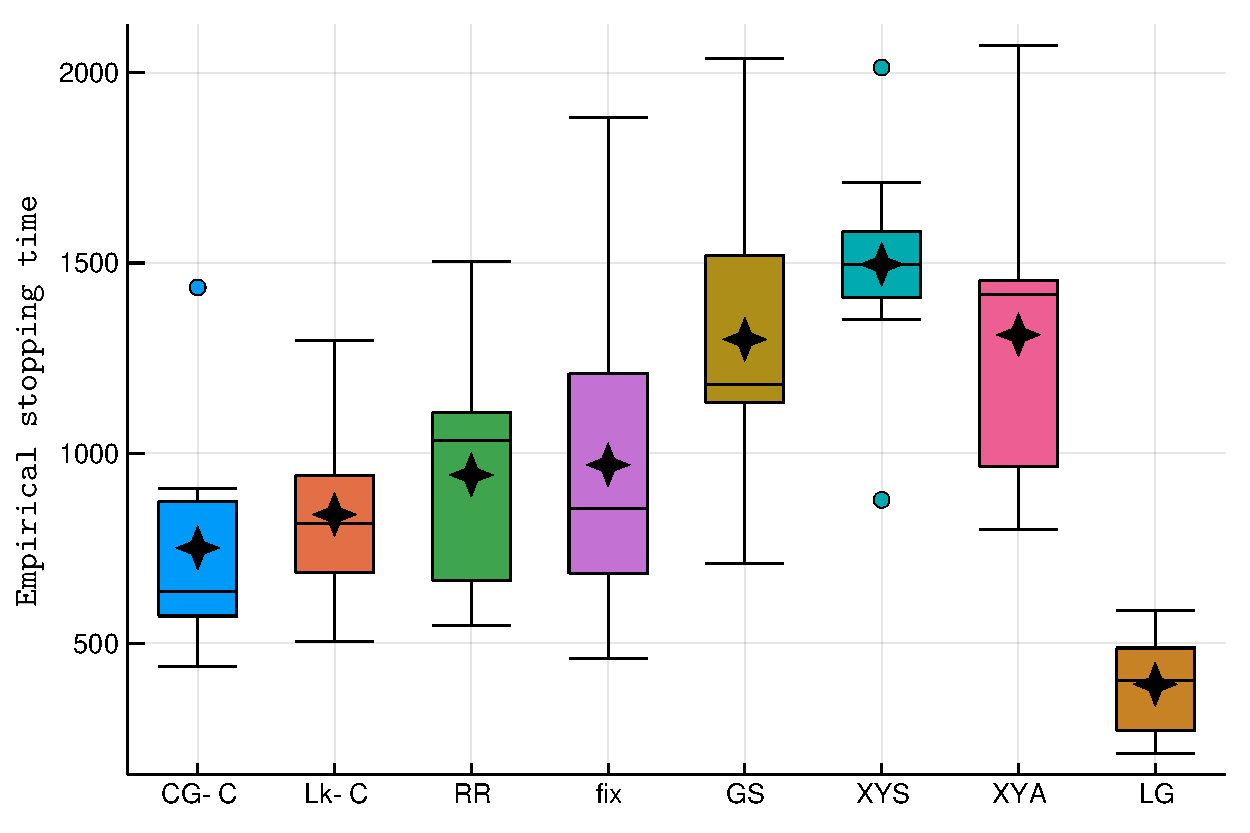
\includegraphics[clip, width= 0.24\textwidth]{Chapter3/img/bai_dim_12}
 \caption{Sample complexity of different linear BAI sampling rules over random unit sphere vectors with $d=6, 8, 10, 12$ from left to right.}
 \label{fig:sample_complexity_2}
\end{figure*}

\section{Experiments}\label{sec:lgc.experiments}
Besides our algorithms, we implement the following algorithms, all using the same stopping rule (more discussion given in Appendix~\ref{app:lgc.stopping}): uniform sampling, the greedy version of \XYS (including $\gopt$-allocation and $\xyopt$-allocation), \XYA, and the greedy version of \LGapE. We skip \GLUCB/\GLGapE since they are more or less equivalent to \LGapE in the scope of this paper.
\vspace{-0.3cm}
\paragraph{The usual hard instance.}
Usual sampling rules for classical BAI may not work for the linear case. This can be understood on a well-studied instance already discussed by~\citet{soare2014linear,xu2018linear}, which encapsulates the difficulty of BAI in a linear bandit, and thus is the first instance on which we test our algorithms. In this instance, arms are the canonical basis  $a_1 = e_1, a_2 = e_2, a_d = e_d$, plus an additional disturbing arm $a_{d+1} = (\cos(\alpha), \sin(\alpha), 0, \ldots, 0)^\top$, and a true regression parameter $\theta$ equal to $e_1$. In this problem, the best arm is always $a_1$, but when the angle $\alpha$ is small, the disturbing arm $a_{d+1}$ is hard to discriminate from $a_1$. As already argued by~\citet{soare2014linear}, an efficient sampling rule for this problem instance would rather pull $a_2$ in order to reduce the uncertainty in the direction $a_1-a_{d+1}$. Naive adaptation of classical BAI algorithms cannot deal with that situation naturally. We further use a simple set of experiments to justify that intuition. We run our two algorithms and the one of~\citet{degenne2019game} that we call \texttt{DKM} over the problem instance whence $d=2$, $\delta=0.01$ and $\alpha=0.1$. We show the number of pulls for each arm averaged over 100 replications of experiments in Table~\ref{table:pulls}. We see that, indeed, \texttt{DKM} pulls too much $a_3$, while our algorithms focus mostly on $a_2$.


\begin{table}[th]\centering
%\def\arraystretch{1.2}
\begin{tabular}{|c|c|c|c|}
 \hline
 & \LG & \LGC & \texttt{DKM} \\
 \hline
 \textbf{$a_1$} & $1912$ & $1959$ & $1943$ \\
 \hline
 \textbf{$a_2$} & $5119$ & $4818$ & $4987$ \\
 \hline
 \textbf{$a_3$} & $104$ & $77$ & $1775$ \\
 \hline
 \textbf{Total} & $7135$ & $\bf{6854}$ & $8705$ \\
 \hline
\end{tabular}
\caption{Average number of pulls of \LG and \LGC (against \texttt{DKM}) for each arm.}
\label{table:pulls}
\end{table}

\vspace{-0.3cm}
\paragraph{Comparison of different complexities.}
We use the previous setting to illustrate various complexities differ in practice. In Table~\ref{table:optimal_weights} we compare the different complexities mentioned in this paper: the characteristic time $\Tstar(\theta)$ and its associated optimal weights $\wstar_{\cA\cBstar(\theta)}$, the $\xyopt$-complexity and its associated optimal design $\wstar_{\xyopt}$, the G-optimal complexity $\gopt$ and its associated optimal design $\wstar_{\cA\cA}$. For each weight vector $w \in\{\wstar_{\cA\cBstar(\theta)},w_{\xyopt}, w_{\gopt}\}$,
 we also provide the lower bound $T_w$ given by Therorem~\ref{th:lb_genral}, i.e.
 \[
 T_w = \max_{a\neq \astar(\theta)} \frac{\big\langle \theta, \astar(\theta)-a\big\rangle^2}{2\normm{\astar(\theta)-a}_{V_w^{-1}}^2} \log(1/\delta).
\]
In particular we notice that targeting the proportions of pulls $w_{\xyopt}, w_{\gopt}$ leads to a much larger lower bound than the one obtained with the optimal weights.
\begin{table}[th]
\centering
%\def\arraystretch{1.2}
\begin{tabular}{|c|c|c|c|}
 \hline
   & $\wstar_{\cA\cBstar}$ & $\wstar_{\xyopt}$  & $\wstar_{\gopt}$   \\
 \hline
 \textbf{$a_1$} & $0.047599$ & $0.499983$ & $0.499983$ \\
 \hline
 \textbf{$a_2$} & $0.952354$ & $0.499983$ & $0.499983$ \\
 \hline
 \textbf{$a_3$} & $0.000047$ & $0.000033$ & $0.000033$ \\
 \hline
 \textbf{$T_w$} & $369$ & $2882$ & $2882$ \\
 \hline
   & $\Tstar(\theta)$ & $2\xyopt/\DeltaMin^2$ & $8\gopt/\DeltaMin^2$\\
 \hline
  \textbf{Complexity} & $0.124607$ & $32.0469$ & $64.0939$ \\
 \hline
\end{tabular}
\caption{Optimal weights for various complexities with $\DeltaMin= 0.0049958$.}
\label{table:optimal_weights}
\end{table}

\paragraph{Comparison with other algorithms.}
Finally we benchmark our two sampling rules against others from the literature. %Note that the main purpose of this paper is to propose algorithms with asymptotic optimality while being practically usable, but we do not claim to have the best performing ones.
We test over two synthetic problem instances, with the first being the previous counter-example. We set $d=2$, $\alpha=\pi/6$. Fig.~\ref{fig:sample_complexity_1} shows the empirical stopping time of each algorithms averaged over 100 runs, with a confidence level $\delta=0.1, 0.01, 0.0001$ from left to right. Our two algorithms show competitive performance (the two leftmost boxes on each plot), and are only slightly worse than \LGapE.

For the second instance, we consider 20 arms randomly generated from the unit sphere $\mathbb{S}^{d-1}\eqdef\{a\in\R^d; \normm{a}_2=1\}$. We choose the two closest arms $a, a'$ and we set $\theta = a + 0.01(a'-a)$ so that a is the best arm. This setting has already been considered by~\citet{tao2018alba}. We report the same box plots over 100 replications as before with increasing dimension in Fig.~\ref{fig:sample_complexity_2}. More precisely, we set $d=6, 8, 10, 12$ respectively, and always keep a same $\delta = 0.01$. Our algorithms consistently show strong performances compared to other algorithms apart from \LGapE. Moreover, we can see that in these random examples, \LGC works better than the non-confexified one, and is even competitive compared to \LGapE.

We stress that although the main focus of this paper is theoretical, with algorithms that are asymptotically optimal, our methods are also competitive with earlier algorithms experimentally.
